\documentclass{bioinfo}
\copyrightyear{2017} \pubyear{2017}

\access{Advance Access Publication Date: Day Month Year}
\appnotes{Application Note}

\usepackage{url}

\begin{document}
\firstpage{1}

\subtitle{Subject Section}

\title[short Title]{Phylotyper: {\it In silico} predictor of subtypes from gene subtypes}
\author[Whiteside \textit{et~al}.]{Matthew D. Whiteside\,$^{\text{\sfb 1,}*}$, Chad R. Laing\,$^{\text{\sfb 1}}$ and Victor P.J. Gannon\,$^{\text{\sfb 1,}*}$}
\address{$^{\text{\sf 1}}$National Microbiology Laboratory, Public Health Agency of Canada, Lethbridge, AB, Canada, T1J 3Z4}

\corresp{$^\ast$To whom correspondence should be addressed.}

\history{Received on XXXXX; revised on XXXXX; accepted on XXXXX}

\editor{Associate Editor: XXXXXXX}

\abstract{\textbf{Summary:} Whole genome sequencing (WGS) is being adopted in public health for improved surveillance and outbreak analysis.
Subtyping; a  is used in public health to infer phenotypes and distinguish bacterial strain groups.
\textit{In silico} tools that predict molecular subtypes from sequences data are needed to transition historical data to WGS-based protocols.
Phylotyper is a novel solution for \textit{in silico} subtype prediction from gene sequences.
Designed for incorporation into WGS pipelines, it is a general prediction tool that can be applied to most molecular subtype schemes.
Phylotyper uses phylogeny to model the evolution of the subtype and infer subtypes for unannotated sequences.
The phylogenic framework in Phylotyper improves accuracy, provides useful contextual feedback, and is more capable of identifying novel subtypes over approaches based solely on sequence similarity.\\
\textbf{Availability and Implementation:} Phylotyper is a python package. It is available from: \url{https://github.com/superphy/insilico-subtyping}.\\
\textbf{Contact:} \href{matthew.whiteside@phac-aspc.gc.ca}{matthew.whiteside@phac-aspc.gc.ca}\\
\textbf{Supplementary information:} Supplementary data are available at \textit{Bioinformatics}
online.}

\maketitle

\section{Introduction}

Whole-genome sequencing (WGS) is transforming the public health field by providing an efficient method for surveying bacterial populations.
The speed, discriminatory power and broad utility of WGS can improve surveillance and outbreak analysis.
Adoption of WGS in public health, however, requires transitioning of historical data with the new methods \citep{Jenkins2015}.
One of the workhorse methods in public health is molecular subtyping (such as serotyping).
As a surveillance tool, subtypes provide a clearcut designation that is typically used to distinguish taxonomic groups and infer phenotypes, for example, pathogens from non-pathogens.
A WGS-based approach to subtyping would have several benefits over current subtype systems; it would be faster, have improved discrimination and would be cheaper and easier to maintain\citep{Jenkins2015}.
Accordingly, new \textit{in silico} tools have been developed to predict subtypes from WGS data \citep{Joensen2015,Ingle2016,CARRILLO2016}.

Phylotyper is a novel \textit{in silico} predictor of subtypes from sequence data. 
Phylotyper is unique in that it builds a phylogenetic tree consisting of reference sequences with known subtype and the unknown query sequences to help inform subtype prediction. 
Using phylogenetic ancestral state reconstruction to assign the likelihood of each subtype to the tree branch points, Phylotyper assigns an unknown query sequence a subtype based on the extrapolated value from its ancestors in the tree.

\section{Implementation}

The core of Phylotyper is an ancestral state reconstruction (ASR) method that has been adapted for hidden state prediction.
In phylogenetic analysis, ancestral state reconstruction involves the prediction of traits of ancestors from existent descendants.
This methodology can be extended to also predict properties in a limited number of existing strains.

In Phylotyper, the \texttt{rerootingMethod} function from the phytools R package is used to perform the ASR \citep{Revell2011}.
This function calculates the maximum marginal likelihood for unknown tip nodes in a phylogenetic tree.
The likelihood reflects the most likely state for the node given the empirically estimated subtype evolution model and phylogeny.
In the context of Phylotyper, the marginal likelihood provides a confidence value associated with a predicted subtype.

Phylotyper is developed in python and R. 
The steps in the Phylotyper pipeline are: 
(1) Identify subtype gene loci in input genomes using BLAST \citep{Camacho2009}.
(2) Align input genes against a pre-aligned set of reference genes using MAFFT's \texttt{--add} feature \citep{Katoh2013}.
(3) If multiple loci are involved, concatenate individual alignments into superalignment.
(4) Generate maximum likelihood phylogenetic tree of aligned genes with FastTree \citep{Price2010}.
(5) Run phytools \texttt{rerootingMethod} using the phylogenetic tree and assigned subtypes \citep{Revell2011}.
(6) Identify the subtype with maximum marginal likelihood for the unknown genes and report to user in text output file.
Users are also provided with an image of the phylogenetic tree overlaid with the likelihood values (e.g. Figure~1\vphantom{\ref{fig:01}}).

\begin{figure}[!tpb]%figure1
\centerline{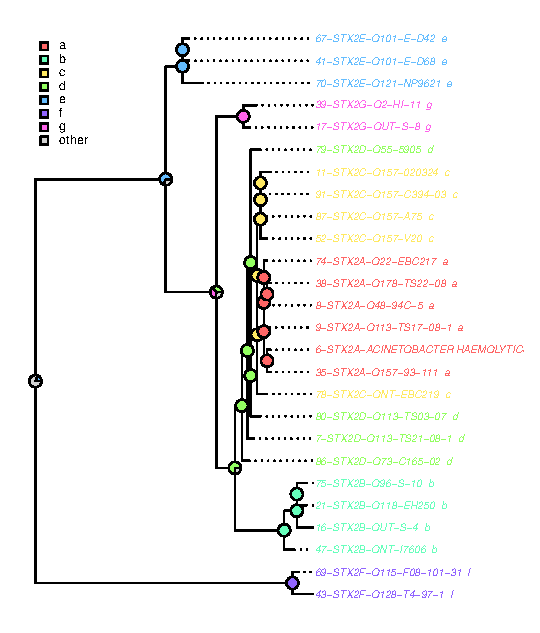
\includegraphics{fig01.eps}}
\caption{Phylogenetic tree for select Stx2 genes. 
The subtype marginal likelihood is displayed at each node as a pie chart.
The full Stx2 tree is displayed in Supplementary Figure S1.}\label{fig:01}
\end{figure}

Phylotyper was designed to be incorporated into a WGS workflow.  
The main input into Phylotyper is assembled genome sequences.  
Putative loci needed for the subtype scheme are identified in the input genomes using BLAST \citep{Camacho2009}.
The identified loci are then sent to the Phylotyper subtype prediction module.
It is possible in Phylotyper to use multiple loci for subtype prediction.
Individual loci alignments are concatenated to form a single superalignment that is used to build the phylogenetic tree.

Currently, subtype schemes for \emph{Escherichia coli} (\textit{E. coli}) are available in the Phylotyper package, and in addition to Stx include intimin and serotype O- and H-types  (Supplementary Table~1).
However, the Phylotyper software also has the capability to add new subtype schemes. 
Creating a new subtype scheme will save the required reference files, allowing newly added schemes to be easily re-run from Phylotyper.
Performance of the Phylotyper method is dependent on the quality of the subtype scheme.
Region / phylogeny is predictive of the subtype
Linkage disequalibrium
homologous genes
Correct alignment and construction of phylogeny
Checks are built-in to the new subtype pipeline to ensure the assumptions of the Phylotyper approach are not violated.  

\section{Results}

Phylotyper marks a progression from the sequence-similarity approach widely used in \it{in silico} subtyping strategies.
It's performance extends beyond allele matching, to perform accurate inference of subtypes for input gene sequences that not in the training data or reference database.
To compare Phylotyper to a sequence similarity-based approach, we ran two validations that looked at how both methods perform when confronted with 1) gene sequence or 2) subtype class not present in the training set.
The first validation was a leave-one-out cross-validation test that iterated through each gene in the training set, retraining the prediction tools on a training set which excludes the selected test gene, and then confirming if the retrained predictor could recover the subtype of the test gene.
This validation tests how the predictors perform when run on a distinct sequence that is not in the training set.
The second validation examined how the predictors respond when presented with a gene that has a subtype not found in the reference set.
In this validation, each subtype was iterated over and all genes that are assigned the subtype were removed from the training set.
In each iteration, we recorded the number of false-positive subtype assignments when the test sequences were used as input.
The correct response for the predictors was to return a negative result, since the subtype does not exist in the training set.
For these assessments, we developed a sequence-similarity based tool that assigns putative subtypes using BLAST.
Details for the BLAST tool and how the assessment was conducted are available in supplementary methods section.
The assessment examined the five subtype schemes available in Phylotyper: Stx1, Stx2, Eae, H-type (FliC), O-type (Wzy \& Wzx).
When tasked with assigning a novel gene sequence (i.e. one that is not in the training set) in the leave-one-out validation, Phylotyper consistently had higher precision than a top-BLAST hit approach.
The average precision in Phylotyper was 0.99 versus 0.96 in the top-BLAST hit approach(result details are available in Supplementary Table S2).
In order to achieve this level of precision, the BLAST approach often had lower recall rates; it had an average recall of 0.81 compared to 0.90 with Phylotyper
Similarily, when entire subtype classes were withheld from the training set, Phylotyper had consistenly lower false positive rates for all subtypes schemes tested; the average precision in this challenging test case was 0.11.
In the BLAST approach, the average precision was 0.30.

A separate assessment for the V-typer tool; a Stx subtype predictor, was run using selected Stx gene sequences from the experimentally-verified Phylotyper training set.
The test Stx genes had sufficent surrounding DNA sequence to support \it{in silico} PCR.
In total, 24 Stx gene sequences were tested with the V-typer tool and V-typer returned results for 7, all correct.
Phylotyper can correctly predict the subtype for all these genes.
Based on this level of recall, it appears the conditions in the Stx subtype setting are challenging for simulated PCR.

\section{Discussion}

From assembled WGS data, Phylotyper can assign unclassifed strains a molecular subtype.
Currently the Phylotyper software offers subtyping schemes for \textit{E. coli}.
It can, however, be applied to most molecular subtype schemes and Phylotyper includes functionality to build new schemes.

Early developers of a serotype predictor for E. coli. This tool uses BLAST.
Performance testing showed that Phylotyper is more robust than an approach based solely on sequence similarity.
The goal of this tool is allele matching, and dependence on reference training set is critical to performance.
To implement allele matching is relatively straight-forward, although some subtyping tools operate with input data such as short reads that require careful analysis.
EcOH uses SRST tool to align and match short reads from ... to known annotated sequences. Again the focus is on matching rather than inference.

Phylotyper computes an empirical model of subtype evolution to predict subtypes for unclassified sequences.
By estimating the phylogenetic distribution of each subtype, Phylotyper is less likely to make type 1 error when encountering a novel subtype. Our empircal testing confirmed this behavior. 
The rate of false positive classifications when we withheld an entire subtype from the training set and used as it the test set was significantly lower than with a straight-forward 

 as one of the subtypes in the database. To validate



or accurately classify a novel sequence allele.
The phylogenetic framework in Phylotyper provides a statistical likelihood for interpreting results.
In comparison, the performance of a sequence similarity approach is highly dependent on the reference database.
This type of approach, there is no inherient mechanism to identify novel alleles.

Subtypes are mainly used as a proxy for evolutionarily-related bacterial strain groups or to infer phenotypes.
Recent analysis of serotype data revealed several inconsistencies between molecular subtype and genomic data \citep{DebRoy2016}.
Subtypes predicted using a phylogenetic framework is more consistent with the main uses of subtype information, so 
Phylotyper is uniquely capable to transition historical subtype data to new WGS systems.\vspace*{-10pt}

\section*{Funding}

This work is funded in part by the Public Health Agency of Canada and a grant from the Genomics Research and Development Initiative\vspace*{-12pt}

\bibliographystyle{natbib}

\bibliography{phylotyper}


\end{document}
